\documentclass[openright,twoside,10pt]{book}

\usepackage[T1]{fontenc}
\usepackage[utf8]{inputenc}

\usepackage{geometry}

\usepackage{amsmath}
\usepackage{amssymb}

\DeclareMathOperator*{\argmax}{arg\,max}
\DeclareMathOperator*{\argmin}{arg\,min}

\usepackage{graphicx}
\graphicspath{ {../img/} }


\usepackage{xcolor}



\usepackage{url}


%\usepackage{cite}
\usepackage[abbr]{harvard}


%\hypersetup{
%    colorlinks=false,
%    linkcolor=blue,
%    filecolor=magenta,      
%    urlcolor=cyan,
%}t

%\urlstyle{same}

\geometry{%
  textwidth  = 156mm ,
  textheight = 234mm ,
  a4paper            ,
  includehead        ,
  hcentering         ,
  vcentering
}

\usepackage[osf,proportional,space]{erewhon}
\usepackage[rigidchapters,pagestyles]{titlesec}
\usepackage{titletoc,lipsum,multicol}

	
\makeatletter
\newcommand\chap@author{}
\newcommand\chapauthor[1]{%
  \cleardoublepage
  \gdef\chap@author{#1}%
}
\def\chap@author{}

\titleformat{\chapter}[hang]
  {\LARGE\bfseries\filright}
  {\thechapter}
  {7pt} % {0pt}	
  {%
    \ifx\chap@author\@empty\else
      \setlength{\unitlength}{1mm}%
      \begin{picture}(0,0)
        \put(0,-17){\makebox(0,0)[l]{\Large\mdseries\itshape \chap@author}}t
      \end{picture}%
    \fi
  }
  [%
    \thispagestyle{empty}%s
    \ifx\chap@author\@empty\else
      \addtocontents{toc}{%
        \vspace{-5pt}%
        \protect\contentsline{chapter}{\mdseries\itshape \chap@author}{}{}%
      }%
      \addtocontents{toc}{\addvspace{5pt}}%
    \fi	
    \startcontents
  ]


\titleformat{\section}[hang]
  {\Large\bfseries\filright}
  {\thesection}
  {7pt} %{0pt} % section title distance between numbering and Title	
  {}

%\titlespacing*{\chapter}{0pt}{0pt}{3cm}
%\titlespacing*{\section}{0pt}{.75pc}{.5pc}s

\titlespacing*{\chapter}{0pt}{0pt}{3cm} % title positions
\titlespacing*{\section}{0pt}{2pc}{.5pc} %{0pt}{0.75pc}{.5pc} % distance from {left margin}{above}{below}
\titlespacing*{\subsection}{0pt}{2pc}{0.5pc}

\newpagestyle{main}{%
  \sethead[%
    \ifx\chap@author\@emptys
      {\makebox[1.5pc][l]{\thepage}{\lsstyle\MakeUppercase\chaptertitle}}%
    \else
      {\makebox[1.5pc][l]{\thepage}{\lsstyle\MakeUppercase\chap@author}}%
    \fi]
    [][]
    {}{}{}
}

\renewcommand\@makefntext[1]{%
  \parindent 1em%
  \noindent
  \hb@xt@1.8em{\hss\@makefnmark\hspace{0.5em}}#1}

\let\footnoterule\relaxs
\makeatother

\usepackage[activate=true]{microtype}
	
\pagestyle{main}

%\setcounter{secnumdepth}{-1}
\setcounter{secnumdepth}{3}

\raggedbottom	


% Hyperref. Hyperref needs to be important last.
%\usepackage{hyperref}
%\hypersetup{s
%    colorlinks = true,
%    linkcolor=blue,
%    linkbordercolor = {blue},
%    citecolor={blue}
%}

\usepackage[
pdfauthor={balthasar},
pdftitle={How to do this},
pdfstartview=XYZ,
bookmarks=true,
colorlinks=true,
linkcolor=blue,
urlcolor=blue,
citecolor=blue,
pdftex,
bookmarks=true,	
linktocpage=true, % makes the page number as hyperlink in table of content
hyperindex=true
]{hyperref}
\usepackage{hyperref}
%\usepackage{harvard}
\urlstyle{rm}
\usepackage[all]{hypcap}
\hypersetup{
backref=true
bookmarksnumbered,
pdfstartview={FitH},
citecolor={blue},
linkcolor={blue},
urlcolor={blue},
pdfpagemode={UseOutlines}
}

\begin{document}
Far from complete and far from correct. These notes exist because I learn better when I express things in my own words. In some cases I might be assembling material for teaching purposes. Might delete later.\\
\\
\texttt{balthasar@rhizomeworks.com}

\tableofcontents
% \chapauthor{J. P. Balthasar Mueller}
\chapter{Combinatorics}

\begin{multicols}{2}[\subsubsection*{Contents of this chapter}]
   \printcontents{}{1}{\setcounter{tocdepth}{2}}
\end{multicols}



\section{Useful Expansions and Identities}



% binomial coefficients
\subsection{Binomial Coefficients and Binomial Expansions}

For two positive integers $n$ and $k$, the binomial coefficient "$n$ choose $k$" is written:

\begin{equation}
{n \choose k} = \left\{ \begin{array}{c} 
\frac{n!}{k!(n-k)!}\ \ \mathrm{for\ }n\geq k\\
\\
0 \ \ \mathrm{otherwise}
\end{array}\right.
\end{equation}

The term can be defined for negative arguments, which is comes up often when working with generating functions.

\begin{equation}
{-n \choose k} = \left\{\begin{array}{c}
(-1)^k { n+k-1 \choose k}\ \ \mathrm{for\ }n\geq k\\
\\
0 \ \ \mathrm{otherwise}
\end{array}\right.
\end{equation}


\begin{equation}
{-n \choose -k} = \left\{\begin{array}{c}
(-1)^{k-n} {k-1 \choose k-n}\ \ \mathrm{for\ }n\geq k\\
\\
0 \ \ \mathrm{otherwise}
\end{array}\right.
\end{equation}

The generalizations are derived in https://arxiv.org/pdf/1105.3689.pdf using symmetry arguments.


% Binomial Expansion
The binomial expansion can be proven either by expanding the polynomial or by creating the Taylor series for the polynomial.

\begin{equation}
(x + y)^n = \sum_{k=0}^n {n \choose k} x^k y^{n-k}
\end{equation}

This holds also for negative integer exponents $n$, in which case:

\begin{equation}
\frac{1}{(y+x)^n} = \sum_{k=0}^\infty {-n \choose k} x^k y^{-n-k} = (-1)^k { n+k-1 \choose k} x^k y^{-(n+k)}
\end{equation}

\subsubsection{Derivation of the Binomial Theorem for a Negative Exponent}

Let $f(x) = \frac{1}{(y+x)^n} = (y+x)^{-n}$. The Taylor expansion about the point $x=0$ is:

\begin{equation}
f(x) = \sum_{k=0}^\infty \frac{f^{(k)}(x=0)}{k!} x^k
\label{eq:taylor}
\end{equation}

The derivatives of $f$ are:

\begin{equation}
\begin{array}{ll}
f^{(0)}(x) &= (y+x)^{-n}\\
f^{(1)}(x) &= (y+x)^{-(n+1)}(-1)n\\
f^{(2)}(x) &= (y+x)^{-(n+2)}(-1)^2 n(n+1)\\
&\vdots\\
f^{(k)}(x) &= (y+x)^{-(n+k)}(-1)^k n(n+1)\hdots	(n+k-1)\\
&=  (y+x)^{-(n+k)}(-1)^k \frac{(n+k-1)!}{(n-1)!}
\end{array}
\label{eq:derivatives}
\end{equation} 

Combing Eqns. \ref{eq:taylor} and \ref{eq:derivatives} gives:

\begin{equation}
f(x) = \sum_{k=0}^\infty (-1)^k {n+k-1 \choose k} x^k y^{-(n+k)}
\end{equation}


\subsubsection{Derivation of the Binomial Theorem for a Fractional Exponent}

Following much the same logic as for a negative exponent, for a fractional exponent the Taylor series is also infinite. 

Let $f(x) = (y+x)^{m}$ with $m\notin \mathbb{Z}$. 

The derivatives of $f$ are:

\begin{equation}
\begin{array}{ll}
f^{(0)}(x) &= (y+x)^{m}\\
f^{(1)}(x) &= (y+x)^{m-1}m\\
f^{(2)}(x) &= (y+x)^{m-2}m(m-1)\\
&\vdots\\
f^{(k)}(x) &= (y+x)^{n-k}m(m-1)\hdots	(m-k+1)\\
\end{array}
\label{eq:derivatives2}
\end{equation} 

Combing Eqns. \ref{eq:taylor} and \ref{eq:derivatives2} gives:

\begin{equation}
f(x) = \sum_{k=0}^\infty { m \choose k } x^k y^{m-k}
\end{equation}

Where, boldly, I defined ${ m \choose k}$ to mean:

\begin{equation}
{m \choose k} = \frac{m(m-1)(m-2)\hdots(m-k+2)(m-k+1)}{k!}
\end{equation}



\subsection{Multinomial Expansion}

\begin{equation}
(x_1 + x_2 + x_3 + \hdots + x_k)^n = \sum_{\begin{array}{c} i_1,i_2,i_3,\hdots,i_k \\ \sum_j i_j = n\end{array}} {n \choose i_1,i_2,\hdots i_k}x^{i_1}x^{i_2}x^{i_3}\hdots x^{i_k}
\end{equation}

with:

\begin{equation}
{n \choose i_1,i_2,\hdots i_k} = \frac{n!}{i_1!i_2!,i_3!\hdots i_k!}
\end{equation}

Where the sum over all possible exponents $i_j$ so that $\sum_j i_j = n$ has ${n+k-1 \choose n}$ terms. 

\subsection{Polynomial Identity}
I don't know what this is called, but it's useful.

\begin{equation}
\prod_i^n (1-x_i) = \sum_{s=0}^{n} (-1)^s \sum_{0\leq \underbrace{i_1,i_2,...,i_s }_{\{i\}_s} \leq n} \prod_{i \in \{i\}_s} x_i
\end{equation}

Where $\{i\}_s$ is a set of $s$ indices that range between $0$ and $n$, and the sum is over all possible such sets, of which there are ${n \choose s}$.  

\subsection{Factorial Expansion}

\begin{equation}
x^{\underline{n}} = \frac{x!}{(x-n)!} = \sum_{k=0}^n s(n,k)x^k
\end{equation}

where

\begin{equation}
s(n,k) = (-1)^{n-k}\left[\begin{array}{c} n\\k \end{array}\right]
\end{equation}

are the stirling numbers of the first kind.

% Stirling Numbers of the second kinds
\section{Stirling Numbers of the Second Kind}
\label{sec:stirling2}

Stirling numbers of the second kind $S(k,n)$ measure the amount of ways in which $k$ objects can be divided into $n$ non-empty groups. They give the number of onto functions from a set of $k$ distinct objects to $n$ indistinct recipients. For example: how many ways can a set of $k$ pool balls be put into $n$ bags, so that there is at least one ball in each bag. All the pool balls have numbers on them and have different colors, so that $n=2$ bags containing $[(1,2,3), (4)] $ and $[(1,2,4),(3)]$ count as different. This sort of problem is discussed at length in section \ref{twentyfoldway}

They are given by an explicit formula:

\begin{equation}
S(k,n) = \frac{1}{n!}\sum_{i=1}^n (-1)^{n-j} {n \choose j}j^k
\end{equation}

They can also be generated via the recurrence relation:

\begin{equation}
\left\{\begin{array}{c}k+1\\n\end{array}\right\} = n\left\{\begin{array}{c}k\\n\end{array}\right\} + \left\{\begin{array}{c}k\\n-1\end{array}\right\}
\end{equation}

The recurrence relation is explained by adding the combinations corresponding to two cases. If the $k+1$st object is added to one of the $n$ existing subsets with $k$ objects, then that corresponds to:

\begin{equation}
n\left\{\begin{array}{c}k\\n\end{array}\right\} = 1
\end{equation}

Possbilities. If the $k+1$st object is in a set by itself (a singleton), then the remaining objects are distributed over $n-1$ set. The combinations arising from this are:

\begin{equation}
\left\{\begin{array}{c}k\\n-1\end{array}\right\} = 1
\end{equation}

Furthermore, the following holds:

\begin{equation}
\left\{\begin{array}{c}0\\0\end{array}\right\} = 1
\end{equation}

\begin{equation}
\left\{\begin{array}{c}k\\0\end{array}\right\} = \left\{\begin{array}{c}0\\n\end{array}\right\} = 0
\end{equation}

And $S(k,n) = 0$ if $n>k$.




% Twentyfold Way
\section{The Twentyfold Way}
\label{twentyfoldway}

The twentyfold way is a taxonomy of distribution problems developed by Kenneth Bogard in his book \textit{Combinatorics through Guided Discovery}. It divides up the way in which $k$ objects may be assigned to $n$ individuals, subject to whether the objects are distinct or identical, and subject to conditions on how the objects are received.


\begin{quote}
\textit{When we are passing out objects to recipients, we may think of the objects as being either identical or distinct. We may also think of the recipients as being either identical (as in the case of putting fruit into plastic bags in the grocery store) or distinct (as in the case of passing fruit out to children). We may restrict the distributions to those that give at least one object to each recipient, or those that give exactly one object to each recipient, or those that give at most one object to each recipient, or we may have no such restrictions. If the objects are distinct, it may be that the order in which the objects are received is relevant (think about putting books onto the shelves in a bookcase) or that the order in which the objects are received is irrelevant (think about dropping a handful of candy into a child?s trick or treat bag). If we ignore the possibility that the order in which objects are received matters, we have created $2\times2\times4 = 16$ distribution problems. In the cases where a recipient can receive more than one distinct object, we also have four more problems when the order objects are received matters. Thus we have 20 possible distribution problems.} - Bogart, \textit{Combinatorics Though Guided Discovery}, Chapter 3.
\end{quote}


What I like about this approach is that the challenge with most of the basic combinatorics problems is to figure out the right way of counting. For this reason, the idea of having a unified handbook-like taxonomy is very appealing. The weakness (in my opinion) is that the language of "objects" and "recipients" is unclear because in practice it's not obvious which is which: if there are $k$ students and $n$ teachers, do the teachers receive students, or do the students receive a teacher? 

A way to resolve this is to say that an object can have only one recipient, but that a recipient might receive more than one object. A more formal path is to think of the act of creating combinations in terms of functions. 

\begin{itemize}
\item The elements of the domain are the objects. 
\item The elements of the range are the recipients. 
\item A function can be many-to-one, but it should not be one-to-many. 
\end{itemize}

\subparagraph{Favorite Teachers} At a school with $k$ students and $n$ teachers, the students all have a favorite teacher. (They might all like the same one.). How many ways are there for all of the $k$ students to pick a favorite? 

\textit{Objects:} $k$ students. \textit{Recipients:} $n$ teachers. Many students might have one favorite teacher. There are $n^k$ combinations. 

\subparagraph{Assembling a Team} Out of a choice of $n$ athletes, a coach must assemble a team of $k$. How many ways are there to form a team? 

\textit{Objects:} n athletes. \textit{Recipients:} team, not on the team. Many athletes can be assigned to one outcome of being on the team or not being on the team. There are ${n \choose k}$ combinations for the team, which is the same number as the ${n \choose n-k}$ selections for the bench. 


% Distinct Objects, No Conditions
\subsection{Distinct Objects, No Conditions on Distributing}


%% Distinct Recipients
\subsubsection{Distinct Recipients}
The $k$ objects are assigned to $n$ recipients with no conditions as to the number of objects each recipient receives. This is the same as assigning the elements of a $k$-tuple from a selection of $n$ \underline{with} replacement.

\begin{equation}	
\begin{array}{l}
S = \{ (a_1,a_2,...,a_k) | a_i \in A, |A| = n \}\\
\\
|S| = n^k
\end{array}
\end{equation}



\subparagraph{Pool Balls into Labeled Buckets} All possible ways to put $k$ pool balls, which all have different numbers and colors, into $n$ labeled buckets. Some of the buckets might be empty, and others might contain more than one of the pool balls.

\subparagraph{Functions} All possible functions $f:x \rightarrow y$ with $\{x | x\in A, |A| = k \}$ and $\{y | y\in B, |B| = n\}$.

\subparagraph{Binary Strings of Length $k$} The $k$ distinct positions of a binary string $(i_1,i_2,...,i_k)$ of length $k$ are assigned to an element of the set $A\in[0,1]$. The number of possible binary strings of length $k$ is $2^k$.

\subparagraph{Subsets of a $k$-Element Set} The subsets of a set of $k$ distinct elements are formed by assigning each of its $k$ distinguishable elements to one of the two labels $A\in [\mathrm{included},\mathrm{excluded}]$. The number of possible subsets, including the empty subset and the full set, is $2^k$.

%% Indistinct Recipients
\subsubsection{Indistinct Recipients}
The $k$ objects are assigned to a recipient that is not distinct. 

\begin{equation}
|A| = \sum_{i=1}^k S(n,i)
\end{equation}

Where $S(k,n)$ is the Stirling number of the second kind that gives the number of ways that $k$ objects can be distributed across $n$ non-empty indistinct sets. The sum above takes care of the case where the $k$ objects are divided into \underline{up to} $n$ collections.  

A closed form expression for the Stirling Numbers of the second kind is (c.f. section \ref{sec:stirling2}): 

\begin{equation}
S(k,n) = \left\{ \begin{array}{c} k \\n \end{array} \right\} = \frac{1}{n!}\sum_{j=0}^n (-1)^{n-j} {n \choose j }j^k
\label{eq:stirling2}
\end{equation}


\subparagraph{Pool Balls into Unlabeled Bags} All possible ways to put $k$ pool balls, which all have different numbers and colors, into $n$ unlabeled bags. Some of the bags might be empty, and others might contain more than one of the pool balls.


% Distinct Objects, At Most One
\subsection{Distinct Objects, Every Recipient Receives At Most One}

%% Distinct Recipients
\subsubsection{Distinct Recipients}
At most one of $k$ distinct objects are assigned to one of $n$ distinct recipients. This is the same as assigning the elements of a $k$-tuple from a selection of $n$ \underline{without} replacement, so that first there are $n$ choices, then $n-1$ choices, $n-2$, etc.

\begin{equation}	
\begin{array}{l}
S = \{ (a_1,a_2,...,a_k) | a_i \in A, |A| = n, a_i\neq a_j\}\\
\\
|S| = \frac{n!}{(n-k)!} = n^{\underline{k}}\ \ \mathrm{if\ }k\leq n,\ 0\ \mathrm{otherwise.}
\end{array}
\end{equation}

\subparagraph{At Most One Pool Ball into Labeled Buckets} All possible ways to put $k$ pool balls, which all have different numbers and colors, into $n$ labeled buckets, but the buckets can have at most one pool ball in them. In other words, you choose any $k$ out of the $n$ labeled buckets and put one pool ball into them. 

\subparagraph{One-to-One Functions} All possible functions $f:x \rightarrow y$ with $\{x | x\in A, |A| = k \}$ and $\{y | y\in B, |B| = n\}$ subject to the constraint that $f(a) = f(b)$ implies $a=b$. That is, the functions are one-to-one, or injective.

\subparagraph{k-element Permutations of $n$ elements}  Each of the $k$ positions in a $k$-element permutation are distinct objects. These are each assigned to one of $n$ possible values, where each value can only show up once. 

\subparagraph{Books on a Shelf} How many ways are there to order $k$ books on a library shelf when there are $n$ different books available. 


%% Indistinct Recipients
\subsubsection{Indistinct Recipients}
At most one of $k$ distinct objects are assigned to one of $n$ indistinct recipients. This is the same as assigning the elements of a $k$-tuple from a selection of $n$ \underline{without} replacement. Except ,since the recipients are all indistinct, there is only one type of choice of recipient for each object. Either each object finds a recipient if $k\leq n$, or it is impossible to distribute at most one object to each recipient because $n < k$.

\begin{equation}
\begin{array}{l}
S = \{ (a_1,a_2,...,a_k) | a_i \in A, |A| = n, a_i=a_j\}\\
\\
|S| = 1\ \ \mathrm{if\ }k\leq n,\ 0\ \mathrm{otherwise.}
\end{array}
\end{equation}



\subparagraph{At Most One Pool Ball into Unlabeled Bags} All possible ways to put $k$ pool balls, which all have different numbers and colors, into $n$ unlabeled bags, but the bags can have at most one pool ball in them. The bags are identical, so the only result is one where there are $k$ bags with a ball in them and $n-k$ without a ball in them. If there are not enough bags, then there is no possible result. 

\subparagraph{Distributing Candy} There are $n$ pieces of identical candy and $k$ kids. How many ways are there to give each kid a piece of candy? If there is enough candy, the answer is one. Everyone gets candy. If there is not enough candy then the answer is zero. There is no way to give everyone candy if there's not enough candy.


% Distinct Objects, At Least One
\subsection{Distinct Objects, Every Recipient Receives at Least One}

%% Distinct Recipients
\subsubsection{Distinct Recipients}

\begin{equation}
|A| = n!S(k,n) =n! \left\{ \begin{array}{c} k \\n \end{array}\right\} = n! \frac{1}{n!}\sum_{j=0}^n (-1)^{n-j} {n \choose j }j^k\end{equation}

Where $S(k,n)$	 denotes the Stirling function of the second kind.


\subparagraph{At Least One Pool Ball into Labeled Buckets} All possible ways to put $k$ pool balls, which all have different numbers and colors, into $n$ labeled buckets, so that all of the buckets have at least one ball in them. This is the same number of combinations as if the buckets were unlabeled, but multiplied with $n!$ ways of applying a label to them.

\subparagraph{Onto Functions} All possible functions $f:x \rightarrow y$ with $\{x | x\in A, |A| = k \}$ and $\{y | y\in B, |B| = n\}$ subject to the constraint that there is an element $x$ in the domain so that $f(x)=y$ for each element $y$ of the codomain. That is the functions are onto, or surjective.


%% Indistinct Recipients
\subsubsection{Indistinct Recipients}
The number of ways to divide $k$ distinct objects into $n$ non-empty subets is given by the Stirling number of the second kind (c.f. section \ref{sec:stirling2}):

\begin{equation}
|A| = S(k,n) = \left\{ \begin{array}{c} k \\n \end{array} \right\} = \frac{1}{n!}\sum_{j=0}^n (-1)^{n-j} {n \choose j }j^k	\end{equation}



\subparagraph{At Least One Pool Ball into Unlabeled Bags} All possible ways to put $k$ pool balls, which all have different numbers and colors, into $n$ unlabeled bags, so that none of the bags are empty. 


% Distinct Objects, Everyone received exactly one
\subsection{Distinct Objects, Every Recipient Receives Exactly One}

% distinct recipients
\subsubsection{Distinct Recipients}
One of $k$ distinct objects are assigned to each of $n$ distinct recipients. This is the same as assigning the elements of a $k$-tuple from a selection of $n$ \underline{without} replacement and with the requirement that all of the $n$ are selected.

\begin{equation}	
\begin{array}{l}
S = \{ (a_1,a_2,...,a_k) | a_i \in A, |A| = k = n, a_i\neq a_j\}\\
\\
|S| = n! = k!\ \ \mathrm{if\ }k=n,\ 0\ \mathrm{otherwise.}
\end{array}
\end{equation}

\subparagraph{Exactly One Pool Ball into Labeled Buckets} All possible ways to put $k$ pool balls, which all have different numbers and colors, into $n$ labeled buckets, that there is one pool ball in each bucket. This is the same as putting one pool ball into unlabeled buckets and multiplying by the $n!$ ways of attaching a label to the buckets. If there isn't the same amount of balls and buckets then there is no possible way for them to be matched one-for-one.

\subparagraph{Bijective Functions} All possible functions $f:x \rightarrow y$ with $\{x | x\in A, |A| = k \}$ and $\{y | y\in B, |B| = n\}$ subject to the constraints that $f(a) = f(b)$ implies $a=b$ and that there is an element $x$ in the domain so that $f(x)=y$ for each element $y$ of the codomain. That is, the functions are one-to-one and onto, of bijective.

\subparagraph{Permutations} Since each of the $k$ objects is given to a different one of the $n$ recipients, there must be as many recipients as there are objects and $k=n$. The number of ways of assigning $k$ objects to $n$ recipients is $k!=n!$.

\subparagraph{Unique Identifiers} Each of $k$ entries in a database is given one of $n=k$ unique identifiers, so that each identifier leads to an entry and each entry has an identifier. 

% indistinct recipients
\subsubsection{Indistinct Recipients}

\begin{equation}	
\begin{array}{l}
S = \{ (a_1,a_2,...,a_k) | a_i \in A, |A| = k, a_i=a_j\}\\
\\
|S| = 1\ \ \mathrm{if\ }k = n,\ 0\ \mathrm{otherwise.}
\end{array}
\end{equation}


\subparagraph{Exactly One Pool Ball into Unlabeled Bags} All possible ways to put $k$ pool balls, which all have different numbers and colors, into $n$ unlabeled bags, that there is one pool ball in each bag. The result is that you either have $n$ bags with $n=k$ balls in them, if the two have matching numbers, or that you either have a bag or a ball left over and there is no way to match them one-for-one.

\subparagraph{Distribute without Leftovers} $k$ students are assigned to $n$ identical textbooks. How many ways are there for each child to have a textbook so that there are no textbooks left over? 


% Distinct Objects, Ordered Groups
\subsection{Distinct Objects, Distributed in Ordered Groups}

\subsubsection{Distinct Recipients}
$k$ objects are distributed to $n$ different recipients with an internal ordering, so that each recipient receives an ordered list. This is the same as creating a list of $n$ sequences that are sampled from $k$ \underline{without replacement}. 

\begin{equation}
\begin{array}{l}
S = \{ (\mathbf{a}_{\{i_1\}}  = ( a_{i_{1,1}},a_{i_{1,1}},...,a_{i_{1,l}} ),\mathbf{a}_{\{i_2\}},...,\mathbf{a}_{\{i_n\}}) | \sum^n_j |\mathbf{a}_{i_j}| = k, a_{i_{j,i}} \in A, |A| = n \} \\
\\
|S| = \frac{(k + n - 1)!}{(n-1)!} = ( k+n-1)^{\underline{k}} = k! {k+n-1 \choose k}
\end{array}
\end{equation}


\subparagraph{Ordered Functions}  All functions $f: x \rightarrow y$ with $\{x | x\in A, |A| = k \}$ and $\{y | y\in B, |B| = n\}$ that assign ordered sequences of elements in $x$ to elements of $y$.

\subparagraph{Labeled Bookshelves} $k$ books are distributed across $n$ different bookshelves. The books may all be on the same shelf, or shelves may be empty. The ordering of the books on each of the shelves matters.


\subsubsection{Indistinct Recipients}
$k$ objects are broken up into $n$ 

\begin{equation}
|S| = \sum_{i=1}^n L(k,i) 
\end{equation}

where $L(k,n)$ are the Lah numbers, which describe "How many ways can $k$ objects be distributed to $n$ recipients if order matters and each recipient receives at least 1". They are given by:

\begin{equation}
L(k,n)= {k \choose n} (k-1)^{\underline{k-n}} = \frac{k!}{n!}{ k-1 \choose n-1 }
\end{equation}

The sum considers the case where all $k$ objects are given to $i\leq n$ recipients, with the remaining recipients receiving none. The expression is more complicated than simply dividing the case for indistinct recipients by $n!$, because more than one of the recipients might receive the same number of objects, in which case i.e. the distribution $[(0),(0),(1,2)]$ would be counted twice.

\subparagraph{Broken Permutations $\leq n$ Parts} The permutations of $k$ distinct elements are ordered sequences of length $k$. If the sequence is cut up into \underline{up to} $n$ different parts of non-zero length, then what results are \textit{broken permutations}.

\subparagraph{Books into Boxes} $k$ different books are put into $n$ identical boxes. How many ways are there to pack the boxes if you keep track of the order in which the books in each box are stacked? 


% Distinct Objects, Distributed in Ordered Groups of At Least One
\subsection{Distinct Objects, Distributed in Ordered Groups of At Least One}

\subsubsection{Distinct Recipients}

\begin{equation}
|S| = \frac{k!}{(k-n)!}\frac{(k-1)!}{(n-1)!} = k^{\underline{n}} (k-1)^{\underline{k-n}}
\end{equation}

\subparagraph{Ordered Onto Functions} All functions $f: x \rightarrow y$ with $\{x | x\in A, |A| = k \}$ and $\{y | y\in B, |B| = n\}$ that assign ordered sequences of elements in $x$ to elements of $y$, where every element $y\in B$ has an assignment of at least one element.

\subsubsection{Indistinct Recipients}
$k$ elements are divided into $n$ ordered sequences of minimum length 1.

\begin{equation}
L(k,n)= {k \choose n} (k-1)^{\underline{k-n}} = \frac{k!}{n!}{ k-1 \choose n-1 }
\end{equation}
	
	
\subparagraph{Broken Permutations $n$ parts} The permutations of $k$ distinct elements are ordered sequences of length $k$. If the sequence is cut up into up to $n$ different parts, then what results are \textit{broken permutations}.

\subparagraph{Books into Boxes} $k$ different books are put into $n$ identical boxes, so that there is at least one book in each box. How many ways are there to pack the boxes if you keep track of the order in which the books in each box are stacked? 


% Identical Objects
\subsection{Identical Objects}

\subsubsection{Distinct Recipients}

\begin{equation}
|S| = {k+n-1 \choose k}
\end{equation}

\subparagraph{Multisets} Multisets are sets in which identical elements might show up several times. For example $\{a,a,b,b,b\}$. They can also be described in terms of the multiplicity of their elements. For example $[a:2, b:3, c:0]$. How many multisets can be formed with $k$ different elements of $n$ different classes?

\subparagraph{Integer Sums} How many different configurations of the $n$ integers $\{ x_i\}_n$ satisfy $x_1 + x_2 + ... + x_n = k$?

\subparagraph{Bosons in Degenerate States} In how many ways might $k$ Bosons populate $n$ degenerate states?


\subsubsection{Indistinct Recipients}

\begin{equation}
|S| = \sum_{i=1}^n P(k,i)
\end{equation}

It turns out that there is no known formula for $P(k,n)$!

\subparagraph{Number Partitions} How many ways are there to divide $k$ objects across \underline{up to} $n$ piles

\subparagraph{Unlabeled Multiplicities of Multisets} For multisets of $k$ elements with $n$ different classes, what is the number of possible multiplicities? For example, a multiset of $k=3$ elements from $n=2$ classes could have multiplicities $[a:3,b:0], [a:2,b:1],[a:1,b:2],[a:0,b:3]$. If we do not care about the labels $a,b$, then the ways that the the $k$ elements migth be distributed are $[3,0]$ and $[2,1]$.

\subparagraph{Boxes of Marbles} $k$ marbles are randomly put into $n$ boxes. How many ways are there for the weight to be distributed among the boxes?



% Identical Objects, Each gets at most one
\subsection{Identical Objects, Each Receives At Most One}

\subsubsection{Distinct Recipients}
$k$ identical objects are distributed across $n$ recipients so that each recipient recieves at most one. That amounts to choosing $k$ out of the $n$ recipients who will receive an object.

\begin{equation}
|S| = { n \choose k}
\end{equation}


\subparagraph{Subsets} $k$ element subsets of a set of size $n$.

\subparagraph{Binary Labels} The problem can also be thought of as assigning a binary label to $n$ elements, where there are $k$ times $1$ and $n-k$ times 0.

\subsubsection{Indistinct Recipients}

\begin{equation}
|S| = 1\ \ \mathrm{if\ }k \leq n,\ 0\ \mathrm{otherwise}
\end{equation}  

\subparagraph{Boxes} How many ways are there to put $k$ marbles in $n$ boxes, if each box is only big enough for one marble. One, if there are enough boxes, or zero, if there aren't enough boxes.


% Identical Everyone Gets At Least one
\subsection{Identical Objects, Each Receives At Least One}

\subsubsection{Distinct Recipients}
This problem is the same as giving each of $n$ recipients one of $k$ objects, and then distributing the remaining $k-n$ objects arbitrarily.  

\begin{equation}
|S| = {k+n-1-k \choose k-n}= {n-1 \choose k-1}
\end{equation}

\subparagraph{Compositions $n$ Parts} How many ways are there to assign $k$ identical objects to $n$ labeled sets of at least one object?

\subsubsection{Indistinct Recipients}

\begin{equation}
|S| = P(k,n)
\end{equation}

It turns out that there is no known formula for $P(k,n)$!

\subparagraph{Partitions in $n$ Parts} How many ways are there to make $n$ piles from $k$ objects.

% Identical Each Gets Exactly one
\subsection{Identical Objects, Each Receives Exactly One}

\subsubsection{Distinct Recipients}

\begin{equation}
|S| = 1\ \ \mathrm{if\ }k = n,\ 0\ \mathrm{otherwise}
\end{equation}  

\subsubsection{Indistinct Recipients}

\begin{equation}
|S| = 1\ \ \mathrm{if\ }k = n,\ 0\ \mathrm{otherwise}
\end{equation}  









% \chapauthor{J. P. Balthasar Mueller}
\chapter{Linear Algebra}

Resolution for the new year: every time you have to look something up, try to make a note of it.

\begin{multicols}{2}[\subsubsection*{Contents of this chapter}]
   \printcontents{}{1}{\setcounter{tocdepth}{2}}
\end{multicols}

\section{Spectral Theorem}

\section{Singular Value Decomposition}





\section{Cholesky Decomposition}
The Cholesky Decomposition exists when a matrix is hermitian and positive-definite. It expresses the matrix $\mathbf{A}$ as:

\begin{equation}
\mathbf{A} = \mathbf{L}\mathbf{L^\dagger}
\end{equation}

Where $\mathbf{L}$ is a lower-triangular matrix with positive, real diagonal entries. The Cholesky decompositions 

\section{Generalized Eigenvectors}

\section{Affine Transformations}

Affine transformations are the combination of a linear map and a translation, which has the form $f(\mathbf{x}) = \mathbf{A}\mathbf{x} + \mathbf{b}$. 

\begin{equation}
f: V \rightarrow W
\end{equation}

Where $V$ and $W$ are vector spaces. Affine transformations can be expresses as matrices by adding an entry with a constant to the vectors that describe a point in space. For example, for $\mathbf{x} \in \mathbb{R}^n$,  the affine transform $f(\mathbf{x}) = \mathbf{A}\mathbf{x} + \mathbf{b}$ with $A\in\mathbb{R}^{n,n}$ and $x,b \in \mathbb{R}^{n}$ can be expressed as the product of a rectangular matrix $\mathbf{M}$ and a vector $\mathbf{c}$ as:

\begin{equation}
\mathbf{A}\mathbf{x} + \mathbf{b} = \underbrace{\left[\begin{array}{c|c} \mathbf{A} & \mathbf{b} \end{array}\right]}_{\mathbf{M}} \underbrace{\left[\begin{array}{c} \mathbf{x} \\ 1\end{array} \right]}_{\mathbf{c}}
\end{equation}

Where $\mathbf{c}^T = \left[x_1,x_2,x_3,...,x_n,1\right]$ and $\mathbf{M} \in \mathbb{R}^{n,n+1}$.

\section{Multilinear Maps}

A multilinear map acts on several vectors in a way that is linear in each of its arguments. A $k$-linear map acts on $k$ vectors, where $k=2$ are bilinear maps and $k=1$ are linear maps.

\begin{equation}	
f: V_1 \times V_2 \times ... \times V_n \rightarrow W
\end{equation}

Where $V_1, V_2, ... , V_n$ and $W$ are vector spaces. An example would be the addition or subtraction of two or more vectors.

\section{Multilinear Forms}
Multilinear forms are multilinear maps that have a scalar output. An example is the dot product between two vectors, or summing over the elements of one or more vectors.

\begin{equation}
f: V_1 \times V_2 \times ... \times V_n \rightarrow K
\end{equation}

Where $V_1, V_2, ... , V_n$ and $K$ is a scalar field.


\section{Types of Matrices}

\subsection{Hermitian}
Hermitian matrices are matrices that are equal to their complex transpose. That is:

\begin{equation}
{\mathbf{A}^{*}}^T = \mathbf{A}^\dagger = \mathbf{A} 
\end{equation}

Hermitian matrices are like a generalization of symmetric matrices to include complex numbers. 

\subsubsection{Properties}
There are many properties. 
\begin{itemize}
\item By definition: $\mathbf{A} = \mathbf{A}^\dagger$
\item Diagonal Entries are all real, since $a_{i,i} = a_{i,i}^*$
\item Inverse is also hermitian:  $\mathbf{A}^{-1} ={ \mathbf{A}^{-1}}^\dagger$
\item Diagonalizable with real eigenvalues and orthogonal eigenvectors $\in \mathbb{C}^n$.
\end{itemize}


\subsection{Triangular}
A lower triangular matrix is a matrix that has all-zero entries above the diagonal.

\begin{equation}
\mathbf{L} = \left[\begin{array}{cccccc} l_{1,1}&&&&&0\\l_{2,1}&l_{2,2}&&&&\\l_{3,1}&l_{3,2}&\ddots&&&\\  \vdots&\vdots&\ddots&\ddots&&\\ \vdots&\vdots&&\ddots&\ddots&\\  l_{n,1}&l_{n,2}&\hdots&\hdots&l_{n,n-1}&l_{n,n}\end{array}\right]
\end{equation}

Upper triangular matrices are matrices that have all-zero entries below the diagonal.

\section{Taking Derivatives}

\begin{equation}
\begin{array}{l}
\frac{d}{d\mathbf{x}} \left(\mathbf{u}^T\mathbf{x}\right) = \left[\frac{d}{dx_1}\left(\sum_i u_i x_i\right),...,\frac{d}{dx_n}\left(\sum_i u_i x_i\right)\right] = \mathbf{u}^T\\
\\
\frac{d}{d\mathbf{x}} \left(\mathbf{x}^T\mathbf{u}\right) = \left[\frac{d}{dx_1}\left(\sum_i u_i x_i\right),...,\frac{d}{dx_n}\left(\sum_i u_i x_i\right)\right] = \mathbf{u}^T\\
\\
\frac{d}{d\mathbf{x}} \left(\mathbf{x}^T\mathbf{x}\right) = \left[\frac{d}{dx_1}\left(\sum_i x_i^2\right),...,\frac{d}{dx_n}\left(\sum_i x_i^2\right)\right] = 2\mathbf{x}^T\\
\\
\frac{d}{d\mathbf{x}} \left(\mathbf{A}x\right) = \left[
\begin{array}{ccc} 
\underbrace{\frac{d}{dx_1}\left(\sum_i A_{1i} x_i\right)}_{A_{11}} &...& \underbrace{\frac{d}{dx_n}\left(\sum_i A_{1i} x_i\right)}_{A_1n}\\
\vdots&\vdots&\vdots\\
\underbrace{\frac{d}{dx_1}\left(\sum_i A_{ni} x_i\right)}_{A_{n1}} &...& \underbrace{\frac{d}{dx_n}\left(\sum_i A_{ni} x_i\right)}_{A_{nn}}\\
\end{array}\right] = \mathbf{A}\\
\end{array}
\end{equation}


\chapauthor{}

\chapter{Probability}

\begin{multicols}{2}[\subsubsection*{Contents of this chapter}]
   \printcontents{}{1}{\setcounter{tocdepth}{2}}
\end{multicols}


\section{Measure Theory}


\section{Functions of Random Variables, Derived Distributions}

(This section needs revision)

I find changes of variables to be the easiest to understand by writing down a joint probability distribution using a delta function to express the conditional probability for the new variables based on the old variables. The next step is to perform a change of variables in the delta function, and integrate. The delta function means that the relationship between the old and the new variables is deterministic. If the relationship is non-deterministic you can use whatever expression for the conditional probability is appropriate.

Let's say that you want to know the probability distribution of the function $\vec{u} = \mathbf{H}(\vec{x})$ of some random variable $\vec{x}$ for which the probability distribution is known.

I personally find it least confusing to approach this problem by thinking about the joint probability distribution, and then obtaining $p(\vec{u})$ through marginalization:

\begin{equation}
p(\vec{u}) = \int dx^n p(\vec{x},\vec{u}) = \int dx^n p_x(\vec{x}) p_u(\vec{u}|\vec{x})
\end{equation}

Since $\vec{u}$ is a deterministic function of $\vec{x}$, the conditional probabiltiy $p_u(\vec{u}|\vec{x}) = \delta(\vec{u} - \mathbf{H}(\vec{x}))$. Explicitly:

\begin{equation}
p(\vec{u}) = \int dx^n p_x(\vec{x}) \delta(\vec{u} - \mathbf{H}(\vec{x}))
\end{equation}

What this does, is to integrate over all the points $p_x(\vec{x})$ where the argument of the delta function is zero. The important thing is that care needs to be taken when the argument of the delta function is itself a function. In that case, a change of variables has to be performed, so that this is no longer the case. On wikipedia, this is done by defining the new variable $du = |\frac{d}{dx}g(x)|dx$, from which follows:

\begin{equation}
\delta(g(x)) = \sum_{x_0} \frac{\delta(x-x_0)}{|g'(x_0)|}
\end{equation}

Where it is necessary to sum over each point $x_0$ for which $g(x_0) = 0$.

Which makes sense. Except, if you rewrite in terms of the new variable, you get an expression that does not strike me as necessarily the same:

\begin{equation}
\int f(x) \delta(g(x))dx = \sum_{n}\int f(g_n^{-1}(u)) \delta(u) \left|\frac{d}{du}g^{-1}(u)\right|du
\end{equation}

Where the sum $n$ is over all functions $g_n^{-1}$ that satisfy $g(g_n^{-1}(u)) = u$. For example, if $u = g(x) = sin(x)$ then $g_n^{-1} = asin(u) + n2\pi$, for any integer $n$. I feel more comfortable with the second path. The answer to my confusion is most likely the inverse function theorem (cf. section \ref{sec:inverse_function_theorem}). In other words: this section needs revision! But hey, I flagged it.

Note that a delta function with a vector argument can be written as a product of the delta functions along each dimension.

Define a new set of variables $\vec{a} = \vec{u} - \mathbf{H}(\vec{x})$. It follows that $\vec{x} = \mathbf{H_n^{-1}}(\vec{u}-\vec{a})$ and the volume element $dx^n = \left| \frac{d}{d\vec{a}}\mathbf{H}_n^{-1}(\vec{u}-\vec{a})\right|da^n$. Here, $H^{-1}_n$ are all the functions that satisfy $\mathbf{H}(\mathbf{H}_n^{-1}(\vec{u})) = \vec{u}$. The integral becomes:

\begin{equation}
p(\vec{u}) = \int da^n p_x(\mathbf{H}^{-1}_n(\vec{u}-\vec{a}))\left| \frac{d}{d\vec{a}}\mathbf{H}_n^{-1}(\vec{u}-\vec{a})\right| \delta(\vec{a})
\end{equation}

At this point it is safe to evaluate the delta function integral. The result is:

\begin{equation}
p(\vec{u}) = p_x(\mathbf{H}^{-1}_n(\vec{u})\left| \frac{d}{d\vec{a}}\mathbf{H}_n^{-1}(\vec{u}-\vec{a})\right|_{(\vec{a}=0)}
\end{equation}

\subsection{Example: Sum of Random Variables}
If the map $\mathbf{H}$ is not bijective, for example because $\vec{u}$ has lower dimensionality than $\vec{x}$, then a bijective map can be artifically constructed by introducing additional variables that are then also marginalized out. For example, if the goal is to calculate the probability of measuring some sum of random variables $s$, then you can define:

\begin{equation}
u_0 = s - \sum(x_i)\\
u_1 = x_1\\
u_2 = x_2\\
\vdots\\
u_{(n-1)} = x_{n-1}
\end{equation}

The inverse is:

\begin{equation}
x_1 = u_1\\
x_2 = u_2\\
\vdots\\
x_n = s - u_0 - \sum_{i<n} x_i
\end{equation}

The argument in the delta function is transformed $\delta(s - \sum(x_i)) \rightarrow \delta(u_0)$. The determinant of the Jacobian $|J| = |\frac{d}{d\vec{u}} H^{-1}(\vec{u})|$ is given by $[\frac{d}{du_1} \mathbf{H^{-1}},\frac{d}{du_2} \mathbf{H^{-1}},...,\frac{d}{du_{n-1}} \mathbf{H^{-1}}]$. That's an $nxn$ matrix where the first row is all $-1$, the lower left is an $(n-1)x(n-1)$ identity matrix, and the lower right is a $(n-1)x1$ vector of 0s. The determinant is one. Consequently the probability distribution of measuring a sum $s$ is given by:

\begin{equation}
p(s)= \int dx^{n-1} p_x(x_1,x_2,x_3,...,s-\sum_{x<n}x_i)
\end{equation}

Which turns out to be the convolution when the variables are independent.

\subsection{Example: Lower Dimensional Random Variable}

This was already the case for the sum of several random variables, in which case the dimensionality of the problem was reduced from many to one. 

Consider the case many to fewer. Again, you just need to perform a change of variables. The new set of variables needs to have the same dimensionality as the old set of variables. The rest should follow pretty obviously. 

Linear example: $\vec{y} = \mathbf{M}\vec{x}$ where $y$ has 2 dimensions and $x$ has 3. 

Transform:

\begin{equation}
u_1 = y_1 - \vec{M_1}\cdot\vec{x}\\
u_2 = y_2 - \vec{M_2}\cdot\vec{x}\\
u_3 = x_3
\end{equation}

You can write this in terms of some invertible matrix $\mathbf{W} = [\mathbf{M},[0,0,1]]$ as $\vec{u} = \mathbf{W}\vec{x}$, so that $dx^n = |\mathbf{W}^{-1}|du^n|$. The integral is then:

\begin{equation}
p(y) = \int du^n p_x(\mathbf{W}^{-1}(\vec{y}-\vec{u}))\delta(u_1)\delta(u_2)|\mathbf{W}^{-1}|
\end{equation}



\section{Copulas}


\section{Relationship Between Distributions}

\chapter{Information Theory}

\begin{multicols}{2}[\subsubsection*{Contents of this chapter}]
   \printcontents{}{1}{\setcounter{tocdepth}{2}}
\end{multicols}

\section{Entropy}

\section{Mutual Information}

\section{Kullback-Leibler Divergence}

\chapter{Stochastic Processes and Time Series Analysis}

\begin{multicols}{2}[\subsubsection*{Contents of this chapter}]
   \printcontents{}{1}{\setcounter{tocdepth}{2}}
\end{multicols}

In the discrete case, time series $X$ is a set of random variables $X = \{X_1, X_2, X_3,...\}$, or alternatively $X = \{X_t: t\in T\}$ where $T$ is the index set. 

\section{Branching Processes}

\section{Markov Chains}
Markov Chains are time series in which the probability of a state depends only on the state preceding it. That is:

\begin{equation}
p(X_{t+1}|X_t, X{t-1},...,X_{1},X_0) = p(X_{t+1}|X_t)
\end{equation}



\section{Martingales}
Martingales are time series in which the expected value of a state is identical to the expected value of the state preceding it. That is:

\begin{equation}
\mathbb{E}X_{t+1} = \mathbb{E}X_{t}
\end{equation}


\subsection{Martingale Convergence Theorem}

\section{Hidden Markov Models}

\section{Ito Calculus}

\section{Chaos Analysis}

\section{Noise}

\subsection{White Noise}
White noise contains all frequencies with the same intensity. That is, it has constant power spectral density. Infinite bandwidth white noise is a purely theoretical concept, but if noise has a flat power spectrum across the frequencies of interest, it is referred to as white noise. 

In discrete time, white noise is a series of uncorrelated random variables with zero mean and finite variance. When the variables all have normal distribution, the noise is referred to as Gaussian white noise. 

\subsection{Gaussian Noise}
Gaussian noise is typically understood to be white noise in which the shocks have a normal distribution.

\subsection{Brownian Noise}
Brownian noise is noise corresponding to random motion (i.e. Brownian motion). The power spectrum is proportional to $\frac{1}{f^2}$.

\section{Empirical Processes}

\section{Mean Field Theory, Fluid Approximation, Deterministic Approximation}
In modeling phenomena with Markov Chain's, the number of elements constituting a system and the possible local states of that system may grow very large. This so-called \textit{state space explosion} is sometimes approached by approximating the system with a continuous state space. Those approaches include \textit{fluid approximation, mean field approximation} or sometimes the \textit{deterministic approximation}. 
\chapter{Statistics}
\label{sec:directionalstats}

\begin{multicols}{2}[\subsubsection*{Contents of this chapter}]
   \printcontents{}{1}{\setcounter{tocdepth}{2}}
\end{multicols}

\section{Directional Statistics}

\subsection{Mean Direction}
The mean direction of a collection of $i$ vectors $\{\mathbf{x}\}_i$ is \cite{damask2019consistent}:

\begin{equation}
\left<\mathbf{x}\right> = \frac{\mathbf{x_s}}{||\mathbf{x_s}||_2}
\end{equation}

Where

\begin{equation}
\mathbf{x_s} = \sum_i \mathbf{x_i}
\end{equation}

The mean vector is not defined in case $||\mathbf{x_s}||_2 = 0$. The alternative way to calculate the mean direction might make use of angles but apparently that creates ambiguity with respect to the choice of a "zero" angle (cf. footnote in \citeasnoun{damask2019consistently}).



\subsection{Dispersion}

Dispersion is a measure of the variance on the direction of a set of vectors $\{\mathbf{x}\}_i$. For a system of vectors, for example an eigenbasis, both common and differential modes of estimation exist. One way of meausuring directional dispersion is to look at the \textit{mean resultant length}:

\begin{equation}
\mu_r = \frac{||\mathbf{x_s}||}{N}\ \ \ 0\leq \mu_r \leq 1
\end{equation}

\textit{Circular variance} may be defined as $\sigma_c = 1-\mu_r$, but apparently there is an issue with generalization to higher dimensions. (TO DO)

An alternative is a model based approach, for example based on the von Mises - Fisher Distribution.

In the case of a basis, \citeasnoun{damask2019consistently} states that, in order to understand the drivers for variation, dispersion parameters should be calculated for each descending subspace of the basis, first including all of the eigenvectors, then excluding the first eigenvector, etc.

% \chapauthor{J. P. Balthasar Mueller}
\chapter{Linear Regression}
\label{chap:linearregression}

\begin{multicols}{2}[\subsubsection*{Contents of this chapter}]
   \printcontents{}{1}{\setcounter{tocdepth}{2}}
\end{multicols}

There is no escaping from linear regression but hardly anyone seems to agree on how to do it properly. Even worse, people seem to expect you to know things like the normal equations, which you'll never, ever need outside of a job interview. 


\section{Ordinary Least Squares}

\subsection{The Normal Equations, Analytical Least Squares Estimator}
Section \ref{sec:linearequations} discussed the case of the linear system of equations:

\begin{equation}
\mathbf{A}\mathbf{x} = \mathbf{b}
\end{equation}


When $\mathbf{A}^{m\times n}$ with $m>n$, so that the system is overdetermined. This is, of course, the starting point for least squares regression, only that the convention is to use different letters:

\begin{equation}
\mathbf{X}\mathbf{\beta} = \mathbf{y}
\end{equation}

And that, seeing that the system is overdetermined, one looks for an approximate solution $\mathbf{\hat{\beta}}$, so that 

\begin{equation}
\mathbf{X}\mathbf{\beta} + \mathbf{\epsilon} = \mathbf{y}
\end{equation}


A natural approach for picking an approximate solution $\mathbf{\hat{\beta}}$ is to look for the projection of $\mathbf{y}$ in the column space of $\mathbf{X}$. That is, since the column rank $\leq n$ of $\mathbf{X}$ is insufficient to express $m$-dimensional $\mathbf{y}$ exactly in terms of only $m$ coefficients $\mathbf{\beta}$, we look for the $n$-dimensional shadow $\mathbf{\hat{\beta}}$ of some hypothetical higher dimensional exact solution. 

The projection has the property that it maximizes the dot product $(\mathbf{X}\mathbf{\hat{\beta}})\cdot \mathbf{y}$, and hence minimizes the length of the difference vector $\epsilon$. In turn, the length of the difference vector $\epsilon$ is $\sqrt{\epsilon\cdot\epsilon}$, which is monotonic to $\epsilon\cdot\epsilon = \sum^m_i \epsilon_i^2$. That means that finding the projection of $\mathbf{y}$ in the column space of $\mathbf{X}$ minimizes the  $L_2$ norm of $\epsilon$, also known as \textit{least squares error}.

There are two ways to go about finding $\mathbf{\hat{\beta}}$.

\subsection{The Quick Way to $\mathbf{\hat{\beta}}$}

By construction, the vector $\epsilon$ is orthogonal to the column space of $\mathbf{X}$. Which means:

\begin{equation}
\begin{array}{rl}
\mathbf{X}^T\epsilon &= 0\\
\mathbf{X}^T\left(\mathbf{X}\mathbf{\hat{\beta}}-\mathbf{y}\right) &= 0\\
\mathbf{X}^T\mathbf{X}\mathbf{\hat{\beta}} &= \mathbf{X}^T\mathbf{y}\\
\mathbf{\hat{\beta}} &= \left(\mathbf{X}^T\mathbf{X}\right)^{-1}\mathbf{X}^T\mathbf{y}
\end{array}
\end{equation}

Making use of the fact that $\mathbf{X}^T\mathbf{X}$ is square and therefore hopefully invertible.

\subsection{The Long Way to $\mathbf{\hat{\beta}}$}

Loss functions play a central role in computational statistics (for example when regularization is introduced), and therefore it is of interest to approach finding $\mathbf{\hat{\beta}}$ by instead minimizing the least square error. This requires:

\begin{equation}
\frac{d}{d\mathbf{\hat{\beta}}}L_2(\epsilon) = 0
\end{equation}

where

\begin{equation}
\begin{array}{rl}
L_2(\epsilon) &= \left(\mathbf{X}\mathbf{\hat{\beta}}-\mathbf{y}\right)^T\left(\mathbf{X}\mathbf{\hat{\beta}}-\mathbf{y}\right)\\
&= \mathbf{\hat{\beta}}^T\mathbf{X}^T\mathbf{X}\mathbf{\hat{\beta}} - \mathbf{\hat{\beta}}^T\mathbf{X}^T\mathbf{y} - \mathbf{y}^T\mathbf{X}\mathbf{\hat{\beta}} + \mathbf{y}^T\mathbf{y}
\end{array}
\end{equation}

Taking derivatives with respect to a vector is covered in section \ref{sec:derivatives}.

It follows:

\begin{equation}
\begin{array}{l}
\frac{d}{d\mathbf{\hat{\beta}}}\left(x^T\mathbf{X}^T\underbrace{\mathbf{X}\mathbf{\hat{\beta}}}_{u(\mathbf{\hat{\beta}})}\right) = \frac{d}{du}\left(u^Tu\right)\frac{d}{d\mathbf{\hat{\beta}}}u = 2u^T\frac{d}{d\mathbf{\hat{\beta}}}u = 2\mathbf{\hat{\beta}}^T\mathbf{X}^T\mathbf{X}\\
\\
\frac{d}{d\mathbf{\hat{\beta}}}\mathbf{\hat{\beta}}^T\mathbf{X}^T\mathbf{y} = \mathbf{y}^T\mathbf{X}\\
\\
\frac{d}{d\mathbf{\hat{\beta}}}\mathbf{y}^T\mathbf{X}\mathbf{\hat{\beta}} = \mathbf{y}^T\mathbf{X}\\
\\
\frac{d}{d\mathbf{\hat{\beta}}}\mathbf{y}^T\mathbf{y} = 0
\end{array}
\end{equation}

So that

\begin{equation}
\begin{array}{rl}
\frac{d}{dx}L_2(\epsilon) = 0 &= 2\mathbf{\hat{\beta}}^T\mathbf{X}^T\mathbf{X} - 2\mathbf{y}^T\mathbf{X}\\
\mathbf{\hat{\beta}}^T\mathbf{X}^T\mathbf{X} &= \mathbf{y}^T\mathbf{X}\\
\mathbf{X}^T\mathbf{X}\mathbf{\hat{\beta}} &= \mathbf{X}^T\mathbf{y}\\
\mathbf{\hat{\beta}} &= \left(\mathbf{X}^T\mathbf{X}\right)^{-1}\mathbf{X}^T\mathbf{y}
\end{array}
\end{equation}



\subsection{Projection Matrix}

If $\mathbf{\hat{y}}=\mathbf{X}\mathbf{\hat{\beta}}$ is the projection of $\mathbf{y}$ in the column space of $\mathbf{X}$, then, based on the result for $\hat{\beta}$, the projection matrix is $\mathbf{P} = \mathbf{X}\left(\mathbf{X}^T\mathbf{X}\right)^{-1}\mathbf{X}^T$. In a fully determined system, $\mathbf{P}=\mathbf{I}$. Projection matrices have eigenvalues that are either $1$ or $0$, corresponding to dimensions that are kept or discarded during the projection operation.


\subsection{Bayesian Perspective on Least Squares Regression}




\subsection{Q-plots}
\subsection{Variance Inflation Factor}



\section{Ridge Regression}
\subsection{Analytical Ridge Estimator}
\subsection{Bayesian Perspective on Ridge Regression}


\chapauthor{}


% \chapauthor{J. P. Balthasar Mueller}
\chapter{Unsupervised Learning}

\begin{multicols}{2}[\subsubsection*{Contents of this chapter}]
   \printcontents{}{1}{\setcounter{tocdepth}{2}}
\end{multicols}

\section{Blind Source Separation}
Blind Source Separation or Blind Signal Separation (BSS) is the separation of mixed signals. An example is the cocktail party problem, where a microphone is recording the conversations of many people speaking at the same time, making the recording unintelligible. Successful BSS would be able to extract the voice of only a single person.  

\section{Clustering}

\subsection{K-Means}
\subsection{Affinity Propagation}

\section{Independent Component Analysis (ICA)}
Independent Component Analysis (ICA) is a decomposition of data into components that have vanishing mutual information. 

\section{Eigenanalysis, Singular Value Decomposition of Data Matrices}
\label{sec:datasvd}

Singular Value Decomposition (SVD) is a matrix decomposition of the form $\mathbf{A}=\mathbf{U}\Sigma\mathbf{V}^T$, where $\mathbf{U}$ and $\mathbf{V}$ are both unitary (cf. section \ref{sec:svd}). The decomposition always exists for a general complex matrix $\mathbf{A}\in\mathbb{C}^{m\times n}$. 
\\

If $\mathbf{X}\in\mathbb{R}^{N\times p}$ is a data matrix with $N$ samples in the rows and $p$ features in the columns, then SVD allows for the decomposition of the data into $p$ linearly independent components, ranked by their explained variance (i.e. their strength in the dataset). The basis of the decomposition turns out the same as for PCA (cf. section \ref{sec:pca}) except that it is arrived at slightly differently, because PCA involves diagonalizing the covariance matrix. The decomposition of the dataset can be understood as follows. In the SVD of the data matrix: 

\begin{equation}
\mathbf{X} = \mathbf{U}\mathbf{\Sigma}\mathbf{V}^T
\end{equation}

The individual rows of $\mathbf{X}$, i.e. the individual data points, are expressed as:

\begin{equation}
\mathbf{x}^T_i = \sum_{j=1}^p u_{i,j}\sigma_j\mathbf{v}_j^T
\end{equation}

Where $\mathbf{x}_i$ is the $i$th data point. Hence the right singular vectors $\mathbf{v}_i$ are the normalized basis vectors, and the columns of $\mathbf{U}$ give the coefficients the basis expansion, together with the singular values $\sigma_i$, which give a measure of the global strength of the corresponding basis vector. 

SVD is scalable to very large datasets and finds many applications in the wild, including page rank, facial recognition, recommendation algorithms etc. 


% eigenfaces
\subsection{Example: Eigenfaces and Facial Recognition}
One famous result are the so-called eigenfaces. The data matrix $\mathbf{X}\in\mathbb{R}^{N\times p}$ consists of $N$ pictures of faces that each have $p$ pixels. The right singular eigenvectors yield $p$ eigenfaces in terms of which any of the $N$ pictures can be expressed. 

Below are the first eigenfaces extracted from the "Labeled Faces in the Wild" dataset, which includes 13233 portraits with 62x47=2914 pixels each. Running SVD on the data matrix $\mathbf{X} \in \mathbb{R}^{13233\times 2914}$ yields the eigenfaces shown in Figure \ref{fig:svd_eigenfaces}.

\begin{figure}
\centering
    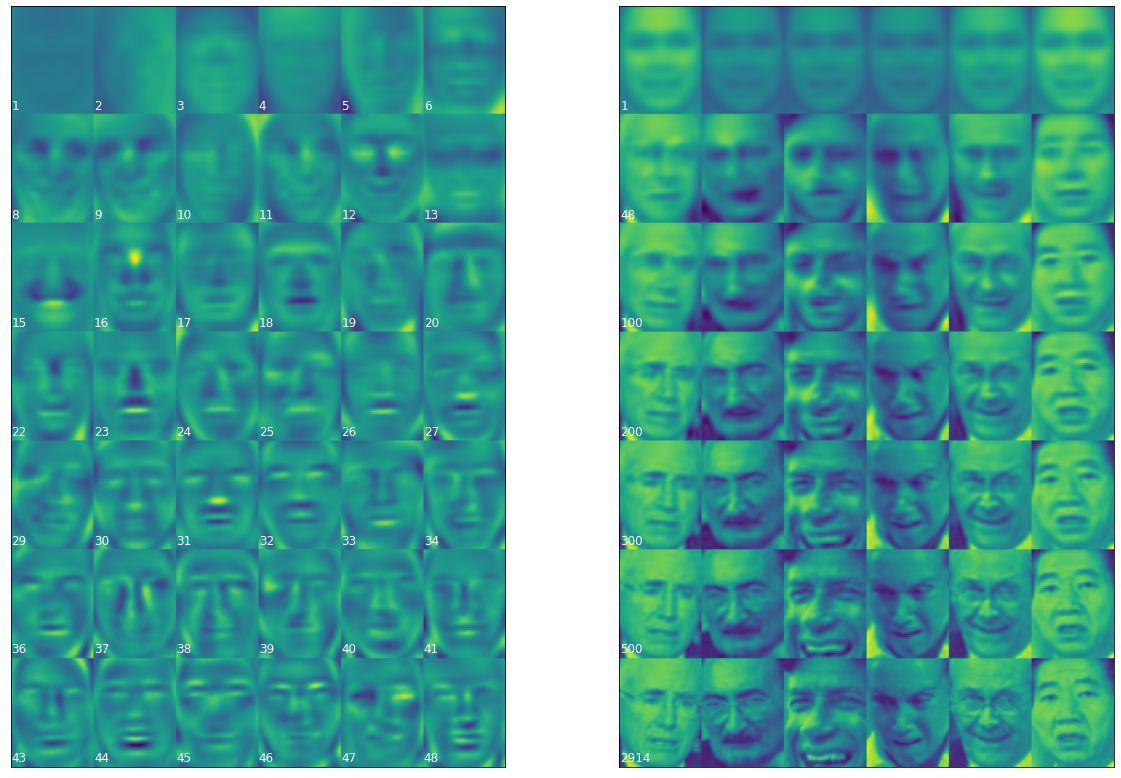
\includegraphics[width=\textwidth]{svd_eigenfaces.png}
    \caption{Left: The first 48 eigenfaces. The colorscale is consistent across the images. As can be expected, the eigenfaces seem to have an ordering from more general features, that are highly prevalent in the dataset, towards more specific features. Right: Five sample portraits from the dataset approximated using different numbers of eigenvectors. 2914 corresponds to the original image, which had 2914 pixels (degrees of freedom).}
    \label{fig:svd_eigenfaces}
\end{figure}

Facial recognition may be performed by projecting a new face into the space of eigenfaces and some form of matching to the coefficients of a known subject. This could be simply the euclidean distance, or it could be a classifier. In case of a classifier, the dimensionality reduction that is enabled by approximating images with a smaller set of eigenvectors may be critical to making the problem tractable by overcoming the curse of dimensionality.


% eigenbasis 
\subsection{Consistently Oriented Eigenbasis}
	
As discussed in section \ref{sec:svd}, the sign of the basis vectors can be flipped without affecting the validity of the singular value decomposition. That means that if the SVD is performed repeatedly on a slowly evolving system, the derived eigenbasis may abruptly change, for example, from a left-handed to a right-handed coordinate system. Hence there is a need to find a way to consistently orient the basis of eigenvectors. A heuristic technique consists of matching the eigenvectors that were derived from two separate decompositions by looking at their dot product, and flipping the signs in order to match them up. A more fundamentally rigorous technique was derived by \citeasnoun{damask2019consistently}. 


% Random SVD
\subsection{Randomized SVD}
\label{sec:rsvd}

Randomized SVD is a method to very efficient and effective way to perform approximate singular value decompositions using random matrix theory. The premise is a very large data matrix $\mathbf{X} \in \mathbb{R}^{n \times m}$ that has low \textit{intrinsic rank} $r$, so that $\mathbf{X} \approx \mathbf{U_r \Sigma_r V_r}^T$ will be a good approximation.

\subsubsection{Step 1: Sample Column Space of $\mathbf{X}$ with $\mathbf{P}$}
Given a random projection matrix $\mathbf{P}\in\mathbb{R}^{m \times r}$, the matrix:

\begin{equation}
\mathbf{Z} = \mathbf{XP}
\end{equation}

will, because of the properties of random matrices, likely have the same rank $r$  dominant column space as $\mathbf{X}$. SVD is usually calculated via the QR-decomposition of a matrix. Performing the QR decomposition of $\mathbf{Z}$ is much less laborious, because $\mathbf{Z}\in\mathbb{R}^{m \times r}$ is much smaller than $\mathbf{X}$. We obtain:

\begin{equation}
\mathbf{X} = \mathbf{QR}
\end{equation}

Where $\mathbf{Q}\in\mathbb{R}^{m \times r}$ and $\mathbf{R}\in\mathbb{R}^{r \times r}$.


\subsubsection{Step 2: Compute SVD on Projected $\mathbf{Y = Q^T X}$}
The next step consists of projecting $\mathbf{Z}$ into $\mathbf{Q}$:

\begin{equation}
\mathbf{Y} = \mathbf{Q}^T\mathbf{X}
\end{equation}

Resulting in the matrix $\mathbf{Y}\in\mathbb{R}^{r\times n}$. Performing the SVD on $\mathbf{Y}$ (which is, again, much smaller than $\mathbf{X}$), gives:

\begin{equation}
\mathbf{Y} = \mathbf{U}_Y\mathbf{\Sigma}_r\mathbf{V}_r^T
\end{equation}

Where $\mathbf{\Sigma}_r$ and $\mathbf{V}_r$ turn out to likely be the same as those that would be obtained from the SVD of $\mathbf{X}$ itself. In the last step, $\mathbf{U}_r$ is recovered using the mathrix $\mathbf{Q}$, via $\mathbf{U}_r = \mathbf{QU}_Y$. 

Guaranteed error bounds for the low rank approximation obtained with this technique. There are two approaches to improve the accuracy of randomized SVD. The first is to oversample, by letting the projection matrix $\mathbf{P}$ have a rank larger than $r$. The second is to "sharpen" the singular value spectrum by using the matrix $\mathbf{(X X^T)^q X }$ instead of $\mathbf{X}$. Calculating the power results in a matrix with a much faster drop off in the singular values, but is much more computationally expensive. This technique is useful when the singular values of $\mathbf{X}$ decay only slowly. The column space of the power iteration $\mathbf{...X X^T X X^T X X^T X}$ has the same column space, so that the trick with the projection operation works here too, only that the dominant subspace will be emphasized.\\


\begin{python}
def rSVD(X,r,q,p):
    """
    Randomized SVD Code
    """
    # Step 1: Sample column space of X with P matrix
    ny = X.shape[1]
    P = np.random.randn(ny,r+p)
    Z = X @ P
    for k in range(q):
        Z = X @ (X.T @ Z)

    Q, R = np.linalg.qr(Z,mode='reduced')

    # Step 2: Compute SVD on projected Y = Q.T @ X
    Y = Q.T @ X
    UY, S, VT = np.linalg.svd(Y,full_matrices=False)
    U = Q @ UY

    return U, S, VT
\end{python}

Empirically, randomized SVD outperforms SVD significantly the lower the rank of the TSVD.


\begin{figure}
\centering
    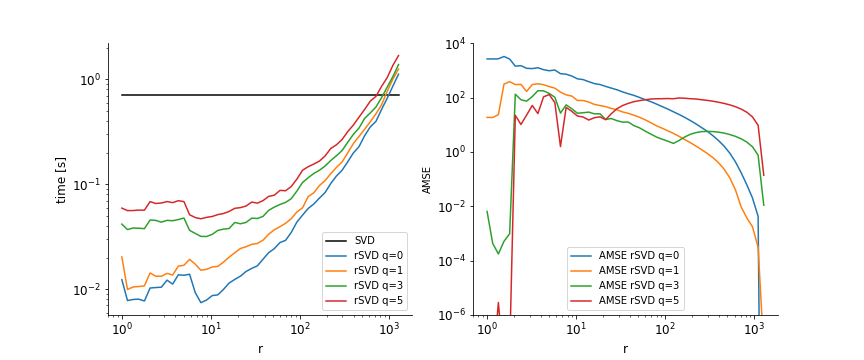
\includegraphics[width=\textwidth]{randomized_svd.png}
    \caption{Left: Time taken to perform conventional SVD (black line) and randomized SVD (colored lines) on the photo of the two young aristocrats which had a data matrix with rank $r=1277$. The different colors correspond to different numbers of power iterations performed ($q$). Right: Average mean square error (AMSE) of truncated SVD using matrices derived with randomized SVD compared with conventional SVD. Especially for small $r$, rSVD is significantly faster even after a few power iterations. For small $r$, power iterations easily reduce the error introduced by the randomized method by several orders of magnitude.}
    \label{fig:svd_scree}
\end{figure}
\section{Principal Component Analysis (PCA)}

Principal Component Analysis (PCA) is a decomposition of data into linearly uncorrelated components. It turns out that these axes are the right-singular eigenvectors $\mathbf{V}$ that are found from SVD. SVD and PCA have close correspondence (cf. section \ref{sec:pcasvd}).
\\

More elaborately, for a data matrix $\mathbf{X}\in\mathbb{R}^{N\times p}$, PCA extracts the ordered, rank-$p$, orthonormal basis in which the $p\times p$ covariance matrix of $\mathbf{X}$ is diagonal. The basis vectors are called the principal axes or principal directions of the data, and their ordering is by the magnitude of the variance that they explain. 
\\

The property that the covariance matrix is diagonal in the principal component basis means that projecting the data onto any of the basis vectors extracts a linearly uncorrelated component of the data that has variance corresponding to the corresponding eigenvalue of the covariance matrix.
\\

Just like with SVD, the ordering of the principal component basis in terms of their explained variance allows for lower-rank approximations of the data matrix to be constructed (section \ref{sec:svd}). Just like SVD, the lower rank approximations $\mathbf{X}$ are the best possible approximations with respect to the Frobenius Norm (cf. section \ref{sec:frobenius}). 
\\

The $p\times p$ covariance matrix  $\mathbf{C}$ of $\mathbf{X}$ is:

\begin{equation}
\mathbf{C} = \frac{\left(\mathbf{X}-\left<\mathbf{X}\right>\right)^T\left(\mathbf{X}-\left< \mathbf{X}\right>\right)}{n-1}
\end{equation}

Where $\left(\mathbf{X}-\left<\mathbf{X}\right>\right)^T$ is often referred to as the \textit{centered} data matrix. The covariance matrix is a symmetric, positive-definite matrix that can be diagonalized with orthonormal eigenvectors $\mathbf{V}$ and positive (or vanishing) eigenvalues $\lambda_i$:

\begin{equation}
\mathbf{C} = \mathbf{V}\mathbf{\Lambda}\mathbf{V}^T
\end{equation}

Where the eigenvectors in $V$ are ordered so that the eigenvectors along the diagonal of $\mathbf{\Lambda}$ have decreasing magnitude. The eigenvectors are the principal axes or principal directions of the data.




\subsection{Relationship between PCA and SVD}
\label{sec:pcasvd}
This is based on a great Stack Exchange answer \cite{amoeba2015svdpca}.

Let the singular value decomposition of the centered data matrix be:

\begin{equation}
\left(\mathbf{X}-\left<\mathbf{X}\right>\right) = \mathbf{U}\mathbf{\Sigma}\mathbf{V}^T
\end{equation}

Then:

\begin{equation}
\mathbf{C} = \frac{\mathbf{V\Sigma U}^T\mathbf{U\Sigma V}^T}{n-1} = \mathbf{V}\frac{\Sigma^2}{n-1}\mathbf{V}^T
\end{equation}

That means that:

\begin{itemize}
\item The principal axes are the right-singular vectors $\mathbf{V}$ that are obtained during SVD.
\item The singular values and the eigenvalues of the covariance matrix are related via $\lambda_i = \frac{\sigma_i^2}{n-1}$.
\end{itemize}


\section{$\mathbf{X}=\mathbf{W}\mathbf{H}$ Non-Negative Matrix Factorization}

Non-Negative Matrix Factorization works for positive matrices and is interesting as a method for dimensionality reduction. It works by expressing a matrix $\mathbf{X}\in\mathbb{R}^{p\times n}_+$ in terms of two smaller positive matrices $\mathbf{W}\in\mathbb{R}_+^{p\times r}$ and $\mathbf{H}\in \mathbb{R}^{r\times n}_+$. An excellent introduction is in \possessivecite{morningpaper2019nnmf} blog post and in \citeasnoun{gillis2014and}. 

Dimensionality reduction derives from the ability to adjust the rank of the decomposition via the dimension $r$.

% Optimal truncation
\section{Optimal Truncation}
\label{sec:truncation}

In any decomposition-based approximation the question emerges of how many terms to keep. The optimal value depends both on the true rank of the underlying signal but also the signal to noise ratio: truncating the decomposition of a rank $r$ data matrix at $r$ does not necessarily give the result that minimizes error. Almost always, the suggestion is to use a heuristic method, but it turns out that one can do better. The discussion below uses the context of singular value decomposition, but the problem of optimal truncation is more general and is an example tuning the hyperparameter that determines the capacity of an estimator to mold itself to a dataset.


\subsection{Scree Plots, Heuristic Methods}
\label{sec:scree}
The canonical heuristic approaches focus on \textit{scree plots}, which simply show the singular values in decreasing order, or cumulative plots, which show the fraction of the total sum of singular values that the first $n$ singular values add up to. In case of PCA, the cumulative plot is directly interpretable as the fraction of the explained variance by the first $n$ principal components, where the total variance is given by $\sigma_2 = \sum_i \sigma_i^2$. \\

A scree plot is sometimes referred to as an \textit{elbow plot}, and a common approach is to truncate at the elbow, which is known as \textit{elbow truncation}. Scree refers to the rock fragments that gather at the foot of a steep hill due to erosion, but I wouldn't really know, because I haven't gone outside in a while. 

Another common way to go about this would be to, for example, keep only the singular components that account to 90\% of the decomposition.

\begin{figure}
\centering
    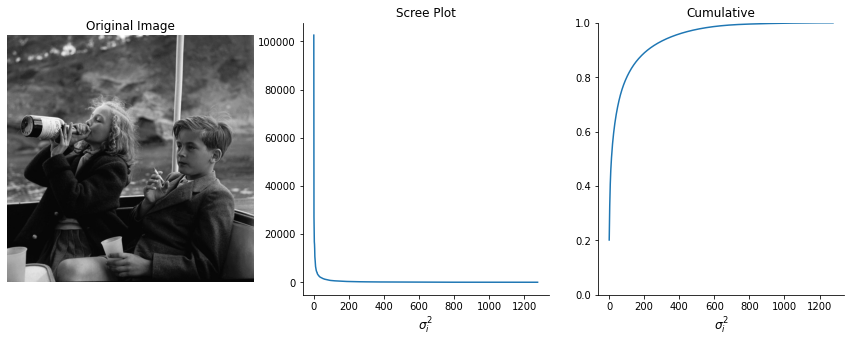
\includegraphics[width=\textwidth]{svd_scree.png}
    \caption{Left: Original image of Princess Yvonne und Prince Alexander zu Sayn-Wittgenstein, photographed by their mother, Princess Marianne, in 1955 (1280 by 1277 pixels). Middle: Scree plot, which shows that the first few components are dominant in the image. Right: Cumulative plot that shows that the first singular component accounts for more than 20\% of the decomposition.}
    \label{fig:svd_scree}
\end{figure}


Either method is not limited to SVD or PCA, but also show up whenever, for example, someone wants to decide on the number of clusters in cluster analysis, the number of regressors in mutlivariate regression (only sometimes), or independent component analysis (ICA).


\subsection{Gavish \& Donoho's Optimal Threshold for SVD}

I came across this through \citeasnoun{gavish2013optimal} and Steve Brunton's youtube channel \cite{stevebrunton}. The idea is the following. Assume that some data matrix $\mathbf{X}\in\mathbb{R}^{N \times p}$ consists of a signal $\mathbf{X}_{r}$ with a rank $r$ substructure, and normally distributed noise with mean zero $\mathbf{X}_{\epsilon}\sim \mathscr{N}(0,\sigma_{\epsilon}^2)$. The method assumes that the rank of the signal $r$ is small compared to the rank of $\mathbf{X}$. 

\begin{equation}
\mathbf{X} = \mathbf{X}_r + \mathbf{X}_{\epsilon}
\end{equation}

The distribution of singular values of a matrix $\mathbf{X}_{\epsilon}\sim \mathscr{N}(0,\sigma_{\epsilon}^2)$ is known up to the variance. \possessivecite{gavish2013optimal} method is to truncate the decomposition of $\mathbf{X}$ at the singular value that fall below the largest singular value of $\mathbf{X}_{\epsilon}$. It turns out that, with respect to average mean square error, this truncation is asymptotically always better than any other truncation and even always better than the true thresholding at rank $r$ when the rank of the underlying signal happens to be known. When the variance of the noise $\sigma^2_{\epsilon}$ is not known, then \citeasnoun{gavish2013optimal} instead use the median singular value of $\mathbf{X}$. 

Let $y_{\mathrm{med}} = \mathrm{med}\{\sigma_i: 1\leq0\leq n\}$ be the median singular value. Then the optimal hard threshold for a matrix $\mathbf{X}\in\mathbb{R}^{m \times n}$ is given by:

\begin{equation}
\tau = \omega(\beta) y_{\mathrm{med}}
\end{equation}

Where $\beta= \frac{m}{n}$ is the aspect ratio of the matrix $\mathbf{X}$ so that $0\leq \beta \leq 1$,  and $\omega(\beta)$ is a constant that needs to be calculated numerically:

\begin{equation}
\omega(\beta) = \frac{\lambda_{*}(\beta)}{\sqrt{\mu_{\beta}}}
\end{equation}

Where $\lambda_{*}(\beta)$:

\begin{equation}
\lambda_{*}(\beta) = \sqrt{2(\beta+1) + \frac{8\beta}{(\beta+1)+\sqrt{\beta^2 + 14\beta+1}}} 
\end{equation}

And $\mu_{\beta}$ is unfortunately the median of the Mar\v{c}enko-Pastur distribution, which is the unique solution to:

\begin{equation}
\int_{\beta_{-}^x}\frac{\sqrt{(\beta_{+}-t)(t-\beta_{-})}}{2\pi t} \mathrm{d}t = \frac{1}{2}
\end{equation}

With $\beta_{\pm} = (1\pm\beta)^2$. Cautiously, \citeasnoun{gavish2013optimal} provide the approximation:

\begin{equation}
\omega(\beta) \approx 0.56\beta^3 - 0.95\beta^2 + 1.82\beta + 1.43
\end{equation}

Which has error bounded by $\leq0.02$ on the interval $0.001\leq\beta \leq 1$.


\begin{figure}
\centering
    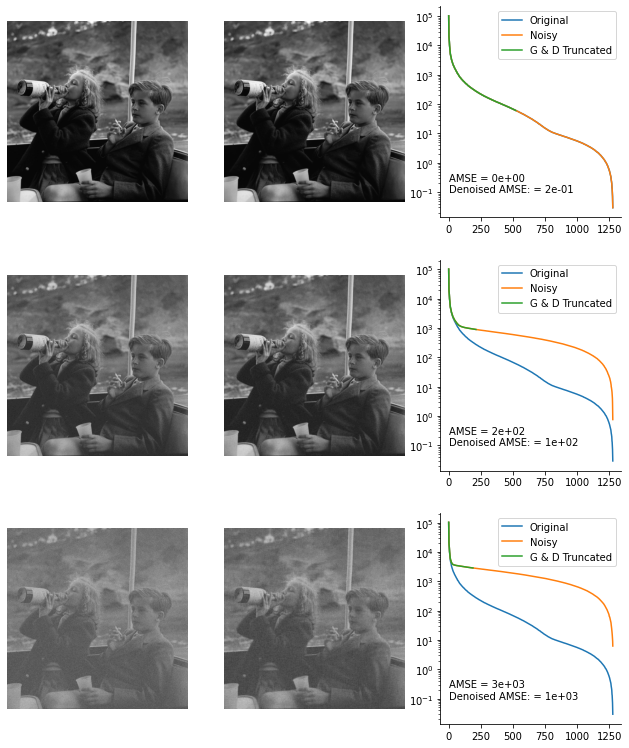
\includegraphics[width=\textwidth]{truncated_svd.png}
    \caption{Left: Princess and Prince zu Sayn-Wittgenstein with different amounts of Gaussian noise added. Center: The same image estimated using TSVD with Gavish \& Donoho's approximate rank threshold. Right: Singular value spectrum of original, noise and truncated images. TSVD reduces the average mean square error (AMSE) with respect to the original image by over 50\%. Visually, the difference is not too perceptible.}
    \label{fig:truncated_svd}
\end{figure}


\chapauthor{}	



\Urlmuskip=0mu plus 2mu\relax
\bibliographystyle{agsm}
\bibliography{references}



\end{document}

